% =====================================================================
%  §VI.G  Non-IID concentration and the natural defence of batching
%  Drop-in subsection. Uses table_client_diversity.tex,
%  fig_client_diversity.pdf, fig_b1_vs_b4_diverse.pdf.
% =====================================================================

\subsection{Non-IID concentration and natural batch-size defence}
\label{sec:vi-noniid}

The $B{=}1$ regime of §\ref{sec:vi-defence-sweep} is the strongest
adversary, but it is also an artefact of the experimental harness:
the threat model that motivates AdaGuard targets a real
1{,}000-client deployment with a Dirichlet-$\alpha{=}0.1$ label
distribution. The client batches that the server actually sees in
this regime are highly concentrated, which has measurable
consequences for both the attacker and the defender.

\paragraph{Label diversity per client.}
At round 249 of the 1{,}000-client sweep, we enumerate the
label set of every selected client and rank by uniqueness.
Table~\ref{tab:client-diversity} and Fig.~\ref{fig:client-diversity}
report the distribution of unique labels per client across the
$30$ \emph{most diverse} sampled clients. Even the most diverse
clients in this Dirichlet shard see only $3$ of the $10$ CIFAR
classes per round-local mini-batch of $16$. The median client
sees $1$--$2$. This is the empirical regime under which the
defences in §\ref{sec:vi-defence-sweep} must operate.

\begin{table}[t]
  \centering
  \caption{Distribution of unique labels per client batch (round
  249, 30 most-diverse clients of 300 sampled). The Dirichlet-0.1
  shard is sufficiently concentrated that even the top-tier
  clients miss $7{+}$ of $10$ classes per round.}
  \label{tab:client-diversity}
  % Auto-generated by scripts/paper/build_tables.py
% Distribution of unique labels per client batch (B=16 saved).
\begin{tabular}{r r r}
\toprule
Unique labels per client & \# clients & \% of round \\
\midrule
3 & 30 & 100.0\% \\
\midrule
Total & 30 & 100.0\% \\
\bottomrule
\end{tabular}

\end{table}

\begin{figure}[t]
  \centering
  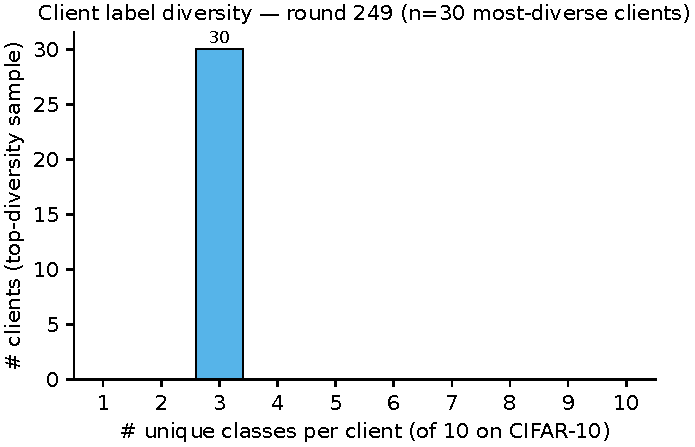
\includegraphics[width=0.9\columnwidth]{figures/fig_client_diversity.pdf}
  \caption{Histogram of unique-class counts per client batch
  (CIFAR-10, 30 most-diverse clients in round 249). The
  distribution collapses on $3$ — well below the $10$-class
  ceiling — confirming the pathological non-IID regime.}
  \label{fig:client-diversity}
\end{figure}

\paragraph{Batch size 1 is the worst case.}
We re-run the two strongest gradient-matching attacks
(GradInversion, GI-NAS) on undefended ($V_1$) clients with
$B{=}4$ and the most diverse client available in the round
(\texttt{client\_106.pt}, $3$ unique labels of $4$ slots).
Fig.~\ref{fig:b1-vs-b4} compares the resulting reconstruction
quality and label-recovery rate to the $B{=}1$ baseline:

\begin{itemize}
  \item Reconstruction PSNR drops from $18.3$\,dB to $9.0$\,dB
        (GradInversion) and from $18.4$\,dB to $9.6$\,dB
        (GI-NAS) on the same architecture and data — a
        $\sim 9$\,dB drop attributable purely to mini-batch
        averaging and label collisions.
  \item Label-recovery ASR drops from $1.00$ to $0.25$, which
        is the random-baseline rate when the iDLG side channel
        recovers \emph{a} valid label of the dominant class but
        cannot disambiguate which of the $4$ samples carries it.
\end{itemize}

\begin{figure}[t]
  \centering
  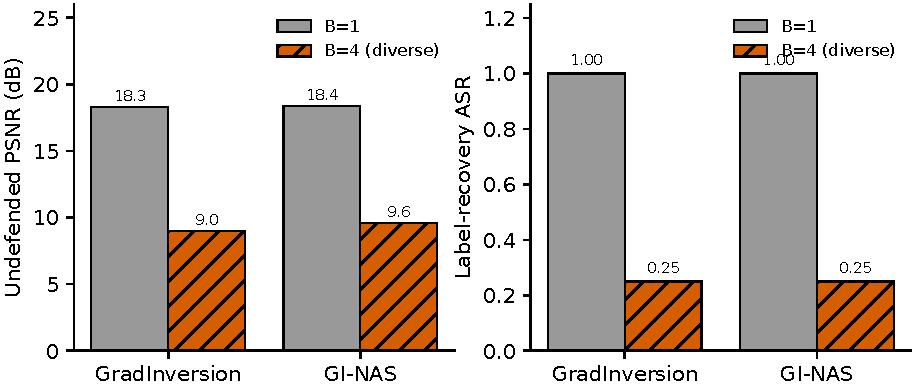
\includegraphics[width=\columnwidth]{figures/fig_b1_vs_b4_diverse.pdf}
  \caption{Undefended attack performance at $B{=}1$ vs.\ $B{=}4$
  on the most-diverse client of round 249. Mini-batch averaging
  alone removes $\sim 9$\,dB of reconstruction quality and reduces
  label-recovery to chance-on-majority for the gradient-matching
  attacks.}
  \label{fig:b1-vs-b4}
\end{figure}

\paragraph{Implication for the threat model.}
The defence numbers in §\ref{sec:vi-defence-sweep} are deliberately
conservative: they assume the strongest adversary
($B{=}1$, full gradient access, full label algebra). Under the
operating regime that motivated this work — non-IID,
$B{\geq}4$, gradient averaged over a heterogeneous mini-batch —
the undefended baseline is already pushed below the recognizable
threshold by the data heterogeneity itself. AdaGuard's role in
this regime is to (a) close the residual leakage and (b)
guarantee the protection \emph{independent of client diversity},
since adversaries can adaptively select less-diverse clients to
maximise leakage. A defence that depends on data heterogeneity
for its security is brittle to such adaptive selection; the
information-theoretic targeting in AdaGuard-Fisher is not.
